%GiG
\documentclass{beamer} 
\usetheme{Copenhagen}
\setbeamertemplate{navigation symbols}{}
\setbeamertemplate{headline}{}
\DeclareMathOperator*{\argmax}{arg\,max}

\usepackage{hyperref}


\definecolor{azure}{rgb}{0.0, 0.5, 1.0}
%\newcommand{\tblue}[1]{\textcolor{blue}{#1}}
\newcommand{\tblue}[1]{{\Large {\textcolor{azure}{#1}}}}
\newcommand{\thblue}[1]{{\Huge {\textcolor{azure}{#1}}}}
\newcommand{\hred}[1]{{\textcolor{red}{#1}}}
\newcommand{\furl}[1]{{\footnote{\url{#1}}}}

\title[Saravanan Thirumuruganathan] 
{Lecture 7: Binary Heaps, Heapsort, Union-Find}

\author[CSE 5311] 
{Instructor: Saravanan Thirumuruganathan}

\date[] 

\begin{document}

\begin{frame}
  \titlepage
\end{frame}

%\begin{frame}{Outline}
%  \tableofcontents
%  % You might wish to add the option [pausesections]
%\end{frame}

\section{Outline}

\begin{frame}
\frametitle {Outline}
\begin{enumerate}
\item Data Structures for representing Dynamic Sets
\begin{itemize}
    \item Binary Heap
    \begin{itemize}
        \item Heapsort
    \end{itemize}
    \item Union Find
\end{itemize}
\end{enumerate}
\end{frame}

\begin{frame}{In-Class Quizzes}
\begin{itemize}
\item {\Large {\bf URL:}} {\LARGE \bf \url{http://m.socrative.com/}} 
\item {\Large {\bf Room Name:} {\LARGE \bf 4f2bb99e}}
\end{itemize}
\end{frame}

\section{General}

\begin{frame}{Data Structures}

\tblue{Key Things to Know for Data Structures}
\begin{itemize}
    \item Motivation
    \item Distinctive Property
    \item Major operations
    \item Key Helper Routines
    \item Representation
    \item Algorithms for major operations
    \item Applications
\end{itemize}
\end{frame}

\section{Binary Heap}
\begin{frame}{}
    \begin{center}
        \thblue{Binary Heap}
    \end{center}
\end{frame}

\begin{frame}{Motivation}
    \begin{itemize}
        \item Heap Sort (CLRS is organized that way!)
        \item Priority Queue
        \item Most space efficient data structure
    \end{itemize}
\end{frame}

\begin{frame}{Priority Queue}
    \begin{itemize}
        \item ``Queue'' data structure has a FIFO property
        \item Some times it is useful to consider {\bf priority}
        \item Output element with highest priority first
    \end{itemize}
\end{frame}

\begin{frame}{Priority Queue - Major Operations}
    \begin{itemize}
        \item Insert
        \item FindMin (resp. FindMax)
        \item DeleteMin (resp. DeleteMax) 
        \item DecreaseKey (resp. IncreaseKey)
    \end{itemize}
\end{frame}

\begin{frame}{Priority Queue - Applications\footnote{{Kleinberg-Tardos Book and Wikipedia}}}
    \begin{itemize}
        \item Dijkstra's shortest path algorithm
        \item Prim's MST algorithm
        \item Heapsort
        \item Online median
        \item Huffman Encoding
        \item A* Search (or any Best first search)
        \item Discrete event simulation
        \item CPU Scheduling
        \item $\ldots$
        \item See Wikipedia entry for priority for details
    \end{itemize}
\end{frame}

\begin{frame}{Priority Queue - Candidate Implementations}
    \begin{itemize}
        \item Assume: for DeleteMin and DecreaseKey, pointer to element is given
        \item LinkedList
        \begin{itemize}
            \item Insert: \pause $O(1)$
            \item FindMin: \pause $O(n)$
            \item DeleteMin: \pause $O(1)$
            \item DecreaseKey: \pause $O(1)$
        \end{itemize}
        \item Binary Heap 
        \begin{itemize}
            \item Insert: $O(\lg n)$
            \item FindMin: $O(1)$
            \item DeleteMin: $O(\lg n)$
            \item DecreaseKey: $O(\lg n)$
        \end{itemize}
        \item Binomial Heaps, Fibonacci Heaps etc.
    \end{itemize}
\end{frame}

\begin{frame}{Binary Heaps}
    \begin{itemize}
        \item Perfect data structure for implementing Priority Queue
        \item MaxHeap and MinHeap
        \item We will focus on MaxHeaps in this lecture
    \end{itemize}
\end{frame}


\begin{frame}{Complete Tree\footnote{\url{http://www.cs.princeton.edu/courses/archive/spring13/cos423/lectures/BinomialHeaps.pdf}}}
    \begin{itemize}
        \item Perfectly balanced, except for bottom level
        \item Elements were inserted top-to-bottom and left-to-right
    \end{itemize}
    \begin{center}
        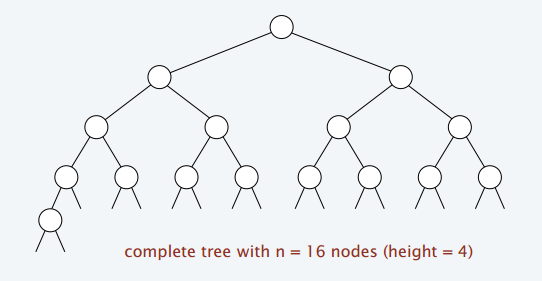
\includegraphics[scale=0.4]{completeTreeEg.png}
    \end{center}
\end{frame}

\begin{frame}{Heap Property}
    \begin{itemize}
        \item Heap is a binary tree ({\bf NOT BST})
        \item Heap:
        \begin{itemize}
            \item {\bf Completeness} Property: Heap has restricted structure. It must be a complete binary tree . 
            \item {\bf Ordering} Property: Relates parent value with that of its children
        \end{itemize}
        \item MaxHeap property: Value of parent must be greater than {\bf both} its children
        \item MinHeap property: Value of parent must be less than {\bf both} its children
        \item Heap with $n$ elements has height $O(\lg n)$
    \end{itemize}
\end{frame}

\begin{frame}{Max Heap Example\footnote{Wikipedia page for Heap}}
    \begin{center}
        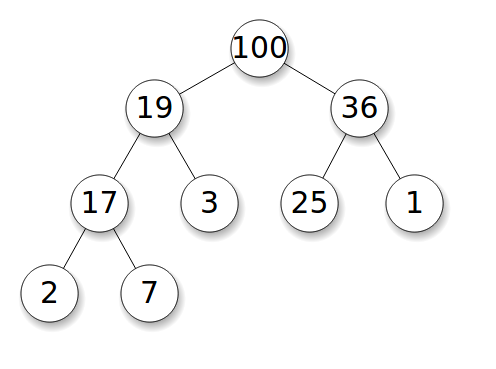
\includegraphics[scale=0.4]{maxHeapEg.png}
    \end{center}
\end{frame}


\begin{frame}{Heap Property\footnote{\url{http://courses.cs.washington.edu/courses/cse373/06sp/handouts/lecture10.pdf}}}
    \begin{center}
        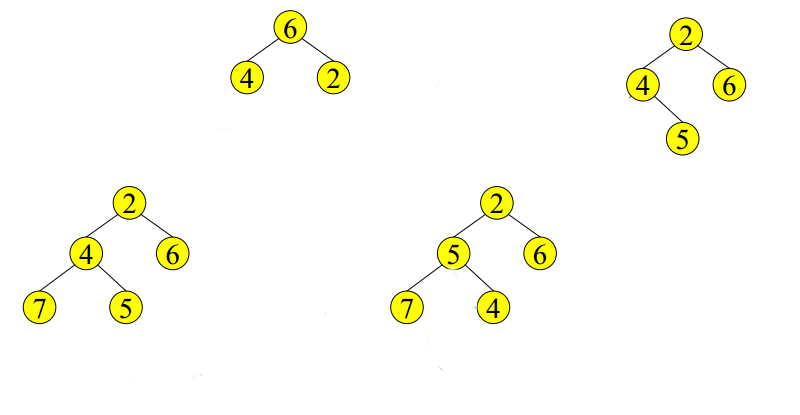
\includegraphics[scale=0.4]{heapOrNot.png}
    \end{center}
\end{frame}

\begin{frame}{Major Operations}
    \begin{itemize}
        \item Insert
        \item FindMax 
        \item DeleteMax (aka ExtractMax)
        \item IncreaseKey
    \end{itemize}
\end{frame}

\begin{frame}{Key Helper Routines}
    \begin{itemize}
        \item Max-Heapify (or Min-Heapify)
        \item Bubble-Up
        \item Bubble-Down
        \item Heapify
    \end{itemize}
\end{frame}

\begin{frame}{Representation: Arrays}
    \begin{itemize}
        \item Very efficient implementation using arrays
        \item Possible due to completeness property
        \item Parent($i$): return $\lfloor i/2 \rfloor$
        \item LeftChild($i$): return $2i$
        \item RightChild($i$): return $2i+1$
    \end{itemize}
\end{frame}

\begin{frame}{Representation: Arrays\footnote{CLRS Fig 6.1}}
    \begin{center}
        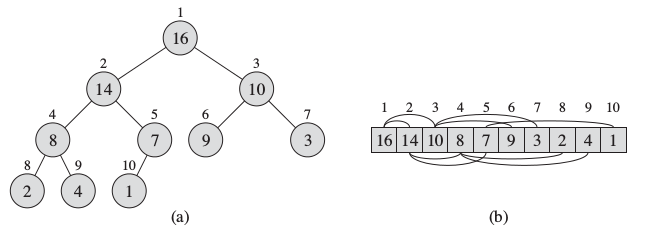
\includegraphics[scale=0.4]{maxHeapRepr.png}
    \end{center}
\end{frame}



\begin{frame}{Max-Heapify}
    \begin{itemize}
        \item Objective: Maintain heap property
        \item Invocation: Max-Heapify($A,i$)
        \item Assume: Left($i$) and Right($i$) are valid max-heaps
        \item $A[i]$ might violate max-heap property
        \item {\bf Analysis:} $O(\lg n)$
    \end{itemize}
\end{frame}


\begin{frame}{Max-Heapify: Example\footnote{CLRS Fig 6.2}}
    \begin{center}
        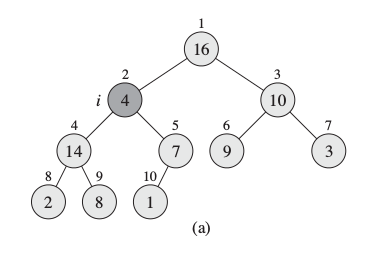
\includegraphics[scale=0.6]{maxHeapify1.png}
    \end{center}
\end{frame}


\begin{frame}{Max-Heapify: Example\footnote{CLRS Fig 6.2}}
    \begin{center}
        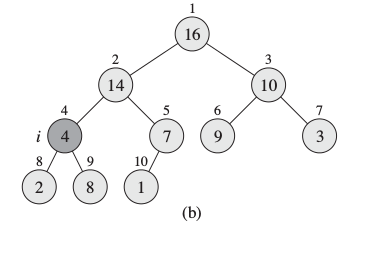
\includegraphics[scale=0.6]{maxHeapify2.png}
    \end{center}
\end{frame}


\begin{frame}{Max-Heapify: Example\footnote{CLRS Fig 6.2}}
    \begin{center}
        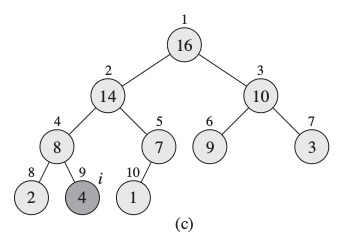
\includegraphics[scale=0.6]{maxHeapify3.png}
    \end{center}
\end{frame}


\begin{frame}{Build-Max-Heap}
    \begin{itemize}
        \item Given an array $A$, convert it to a max-heap
        \item $A.length$: Length of the array
        \item $A.heapSize$: Elements from 1 $\ldots$ A.heapSize form a heap
        \item Build-Max-Heap($A$):
        \begin{itemize}
            \item A.heapSize = A.length
            \item for $i = \lfloor A.length / 2 \rfloor$ down to $1$ \\ \qquad Max-Heapify($A,i$)
        \end{itemize}
        \item {\bf Analysis:} $O(n)$
    \end{itemize}
\end{frame}


\begin{frame}{Build-Max-Heap : Example \footnote{CLRS Fig 6.3}}
    \begin{center}
        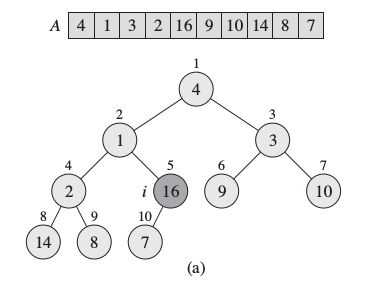
\includegraphics[scale=0.5]{buildMaxHeap1.png}
    \end{center}
\end{frame}


\begin{frame}{Build-Max-Heap : Example \footnote{CLRS Fig 6.3}}
    \begin{center}
        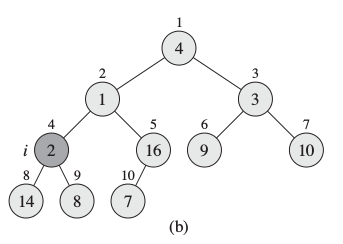
\includegraphics[scale=0.5]{buildMaxHeap2.png}
    \end{center}
\end{frame}


\begin{frame}{Build-Max-Heap : Example \footnote{CLRS Fig 6.3}}
    \begin{center}
        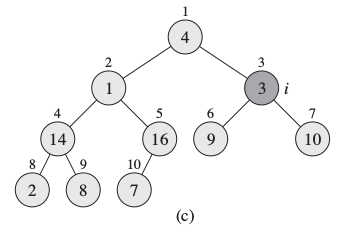
\includegraphics[scale=0.5]{buildMaxHeap3.png}
    \end{center}
\end{frame}


\begin{frame}{Build-Max-Heap : Example \footnote{CLRS Fig 6.3}}
    \begin{center}
        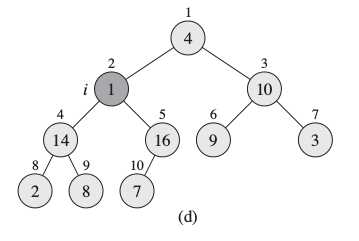
\includegraphics[scale=0.5]{buildMaxHeap4.png}
    \end{center}
\end{frame}


\begin{frame}{Build-Max-Heap : Example \footnote{CLRS Fig 6.3}}
    \begin{center}
        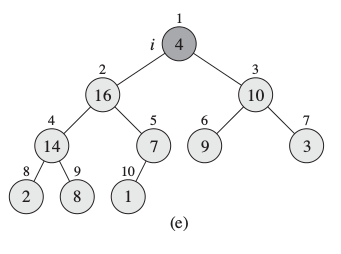
\includegraphics[scale=0.5]{buildMaxHeap5.png}
    \end{center}
\end{frame}


\begin{frame}{Build-Max-Heap : Example \footnote{CLRS Fig 6.3}}
    \begin{center}
        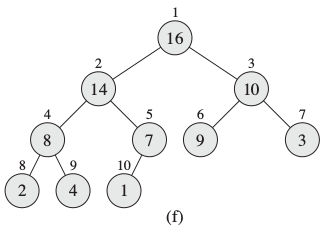
\includegraphics[scale=0.5]{buildMaxHeap6.png}
    \end{center}
\end{frame}


\begin{frame}[fragile]{HeapSort}
    \begin{verbatim}
    HeapSort(A):
        Build-Max-Heap(A)
        for i = A.length down to 2
            Exchange A[1] with A[i]
            A.heapSize = A.heapSize - 1
            Max-Heapify(A, 1)
    \end{verbatim}
\end{frame}


\begin{frame}{Heap Sort: Example\footnote{CLRS Fig 6.4}}
    \begin{center}
        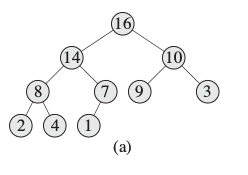
\includegraphics[scale=0.5]{heapSort1.png}
    \end{center}
\end{frame}


\begin{frame}{Heap Sort: Example\footnote{CLRS Fig 6.4}}
    \begin{center}
        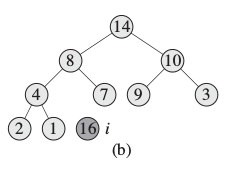
\includegraphics[scale=0.5]{heapSort2.png}
    \end{center}
\end{frame}


\begin{frame}{Heap Sort: Example\footnote{CLRS Fig 6.4}}
    \begin{center}
        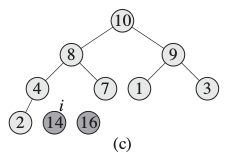
\includegraphics[scale=0.5]{heapSort3.png}
    \end{center}
\end{frame}


\begin{frame}{Heap Sort: Example\footnote{CLRS Fig 6.4}}
    \begin{center}
        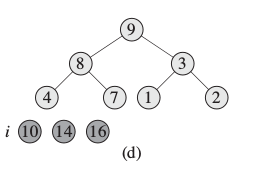
\includegraphics[scale=0.5]{heapSort4.png}
    \end{center}
\end{frame}


\begin{frame}{Heap Sort: Example\footnote{CLRS Fig 6.4}}
    \begin{center}
        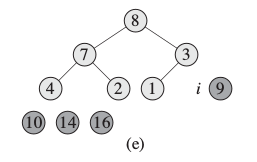
\includegraphics[scale=0.5]{heapSort5.png}
    \end{center}
\end{frame}


\begin{frame}{Heap Sort: Example\footnote{CLRS Fig 6.4}}
    \begin{center}
        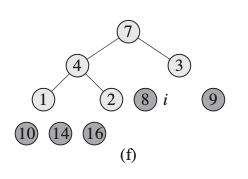
\includegraphics[scale=0.5]{heapSort6.png}
    \end{center}
\end{frame}


\begin{frame}{Heap Sort: Example\footnote{CLRS Fig 6.4}}
    \begin{center}
        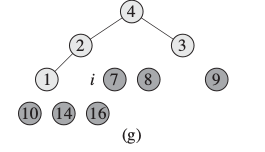
\includegraphics[scale=0.5]{heapSort7.png}
    \end{center}
\end{frame}


\begin{frame}{Heap Sort: Example\footnote{CLRS Fig 6.4}}
    \begin{center}
        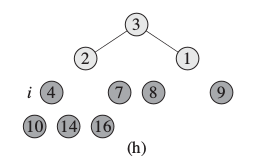
\includegraphics[scale=0.5]{heapSort8.png}
    \end{center}
\end{frame}


\begin{frame}{Heap Sort: Example\footnote{CLRS Fig 6.4}}
    \begin{center}
        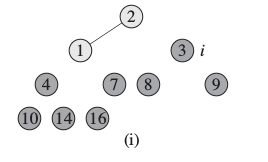
\includegraphics[scale=0.5]{heapSort9.png}
    \end{center}
\end{frame}


\begin{frame}{Heap Sort: Example\footnote{CLRS Fig 6.4}}
    \begin{center}
        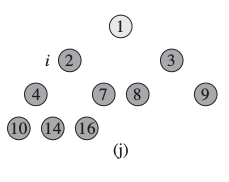
\includegraphics[scale=0.5]{heapSort10.png}
    \end{center}
\end{frame}


\begin{frame}{Heap Sort: Example\footnote{CLRS Fig 6.4}}
    \begin{center}
        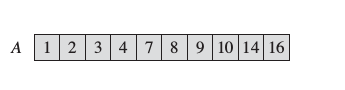
\includegraphics[scale=0.5]{heapSort11.png}
    \end{center}
\end{frame}


\begin{frame}{}
    \begin{itemize}
        \item GiG
    \end{itemize}
\end{frame}


\section{Heapsort}
\section{Union-Find}
\section{Summary}

\begin{frame}{Summary}

\tblue{Major Concepts:}
\begin{itemize}
\item Binary Heap
\item Heapsort
\item Union-Find
\end{itemize}
\end{frame}


\end{document}

